\documentclass[a4paper,12pt]{article}
\usepackage{float}
\usepackage{amsmath, amssymb}
\usepackage{graphicx}
\usepackage{multirow}
\usepackage{booktabs}
\usepackage{geometry}
\usepackage{enumitem}
\usepackage{listings}
\usepackage{xcolor}
\usepackage{tikz}
\geometry{margin=1in}

\usepackage[numbers]{natbib}
\usepackage{multicol}
\usepackage[bookmarks=true]{hyperref}
\usepackage[font=footnotesize]{subfig}
\usepackage{mathtools}
\usepackage[labelfont=bf]{caption}
\usepackage{wrapfig}
\usepackage[ruled,vlined]{algorithm2e}

\begin{document}

\begin{center}
    \Large \textbf{Assignment 2} \\[6pt]
    2025.11.17
\end{center}

\section*{A. Forward Kinematics }
\subsection*{1. Compute the DH parameters}
\begin{table}[h!]
\centering
\begin{tabular}{c|c|c|c|c}
\hline
$i$ & $\alpha_{i-1}$ & $a_{i-1}$ & $d_i$ & $\theta_i$ \\ \hline
1   &       0        &     0     &   0   &   $q_1$    \\ \hline
2   &       0        &   $L_1$   &   0   & $q_2 - \pi/2$ \\ \hline
3   &       0        &   $L_2$   &   0   &   $q_3$    \\ \hline
4(E) &      0        &   $L_3$   &   0   &      0     \\ \hline
\end{tabular}
\caption{DH parameters for the 3-DoF RRR Puma}
\end{table}

\subsection*{2. Transformation between frames}
The general DH transformation is:
\[
{}^{i-1}_{i}T =
R_x(\alpha_{i-1})\, T_x(a_{i-1})\, R_z(\theta_i)\, T_z(d_i).
\]
Homogeneous transformations matrix:
\[
{}^{i-1}_{i}T =
\begin{bmatrix}
\cos\theta_i & -\sin\theta_i & 0 & a_{i-1} \\
\sin\theta_i \cos\alpha_{i-1} &
\cos\theta_i \cos\alpha_{i-1} &
-\sin\alpha_{i-1} &
-\sin\alpha_{i-1} d_i \\
\sin\theta_i \sin\alpha_{i-1} &
\cos\theta_i \sin\alpha_{i-1} &
\cos\alpha_{i-1} &
\cos\alpha_{i-1} d_i \\
0 & 0 & 0 & 1
\end{bmatrix}
\]

\[
{}^{0}_{1}T=
\begin{bmatrix}
c_1 & -s_1 & 0 & 0 \\
s_1 & c_1 & 0 & 0 \\
0 & 0 & 1 & 0\\
0&0&0&1
\end{bmatrix}
\]

\[
{}^{1}_{2}T=
\begin{bmatrix}
s_2 & c_2 & 0 & L_1 \\
-c_2 & s_2 & 0 & 0 \\
0 & 0 & 1 & 0 \\
0&0&0&1
\end{bmatrix}
\]

\[
{}^{2}_{3}T=
\begin{bmatrix}
c_3 & -s_3 & 0 & L_2 \\
s_3 & c_3 & 0 & 0 \\
0 & 0 &1 &0\\
0&0&0&1
\end{bmatrix}
\]

\[
{}^{3}_{E}T=
\begin{bmatrix}
1&0&0&L_3\\
0&1&0&0\\
0&0&1&0\\
0&0&0&1
\end{bmatrix}
\]

End-effector transform
\[
{}^{0}_{E}T = {}^{0}_{1}T\, {}^{1}_{2}T\, {}^{2}_{3}T\, {}^{3}_{E}T
\]

After simplification:

\[
{}^{0}_{E}T=
\begin{bmatrix}
s_{123} & c_{123} & 0 &
L_1 c_1 + L_2 s_{12} + L_3 s_{123} \\
-c_{123} & s_{123} & 0 &
L_1 s_1- L_2 c_{12} - L_3 c_{123} \\
0 & 0 & 1 & 0 \\
0 & 0 & 0 & 1
\end{bmatrix}
\]

where  
\[
s_{12}=s_1 c_2 + c_1 s_2, \quad
c_{01}=c_1 c_2 - s_1 s_2,
\]
\[
s_{123}= s_{12} c_3 + c_{12}s_3,\quad
c_{123}=c_3 c_{12}-s_3 s_{12}.
\]

\subsection*{3. End effector position in Operational space}
\[
F(q)=
\begin{bmatrix}
L_1 c_1 + L_2 s_{12} + L_3 s_{123} \\
L_1 s_{1} - L_2 c_{12} - L_3 c_{123} \\
q_1 + q_2 + q_3 - \frac{\pi}{2}                                             
\end{bmatrix}
\]

\subsection*{4. Compute the End Effector Jacobian}
\[
J(q)=
\dfrac{\partial F(q)}{\partial q}=
\begin{bmatrix}
-L_1 s_1 + L_2 c_{12} + L_3 c_{123} & L_2 c_{12} + L_3 c_{123} & L_3 c_{123} \\
L_1 c_{1} + L_2 s_{12} + L_3 s_{123} &  L_2 s_{12} + L_3 s_{123} &  L_3 s_{123} \\
1 & 1 &1                                            
\end{bmatrix}
\]

\subsection*{5. Understanding the Jacobian Matrix and Pose Singularities}
\subsubsection*{i) \quad $q_1 = (0,0,-\frac{\pi}{2})^T$}
\begin{figure}[h!]
\centering
% ----------------- First figure -----------------
\begin{minipage}{0.32\textwidth}
\centering
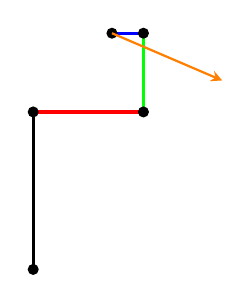
\begin{tikzpicture}[scale=2, >=stealth]
\coordinate (O) at (0,0);
\coordinate (A) at (0,1);
\coordinate (B) at (0.7,1);
\coordinate (C) at (0.7,1.5);
\coordinate (D) at (0.5,1.5);
\draw[black, very thick] (O) -- (A);
\draw[red,   very thick] (A) -- (B);
\draw[green, very thick] (B) -- (C);
\draw[blue,  very thick] (C) -- (D);
\foreach \p in {O,A,B,C,D}{
    \fill (\p) circle (1pt);
}
\draw[->, orange, thick] (D) -- ++(0.7,-0.3);
\end{tikzpicture}
\vspace{3pt}

\(\dot{q} = (1,0,0)\)
\end{minipage}
\hfill
% ----------------- Second figure -----------------
\begin{minipage}{0.32\textwidth}
\centering
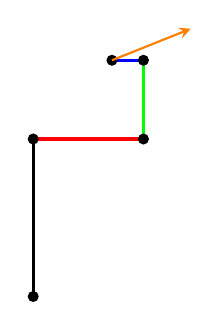
\begin{tikzpicture}[scale=2, >=stealth]
\coordinate (O) at (0,0);
\coordinate (A) at (0,1);
\coordinate (B) at (0.7,1);
\coordinate (C) at (0.7,1.5);
\coordinate (D) at (0.5,1.5);
\draw[black, very thick] (O) -- (A);
\draw[red,   very thick] (A) -- (B);
\draw[green, very thick] (B) -- (C);
\draw[blue,  very thick] (C) -- (D);
\foreach \p in {O,A,B,C,D}{
    \fill (\p) circle (1pt);
}
\draw[->, orange, thick] (D) -- ++(0.5,0.2);
\end{tikzpicture}
\vspace{3pt}

\(\dot{q} = (0,1,0)\)
\end{minipage}
\hfill
% ----------------- Third figure -----------------
\begin{minipage}{0.32\textwidth}
\centering
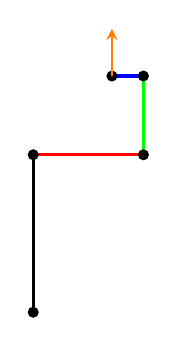
\begin{tikzpicture}[scale=2, >=stealth]
\coordinate (O) at (0,0);
\coordinate (A) at (0,1);
\coordinate (B) at (0.7,1);
\coordinate (C) at (0.7,1.5);
\coordinate (D) at (0.5,1.5);
\draw[black, very thick] (O) -- (A);
\draw[red,   very thick] (A) -- (B);
\draw[green, very thick] (B) -- (C);
\draw[blue,  very thick] (C) -- (D);
\foreach \p in {O,A,B,C,D}{
    \fill (\p) circle (1pt);
}
\draw[->, orange, thick] (D) -- ++(0, 0.3);
\end{tikzpicture}
\vspace{3pt}

\(\dot{q} = (0,0,1)\)
\end{minipage}
\end{figure}
\noindent
The configuration is \textbf{not a singularity}, based on the direction and independence of the end-effector velocity vectors, it can move in x- and y-direction.

\subsubsection*{ii) \quad $q_2 = (-\frac{\pi}{2},\frac{\pi}{2},0.1)^T$}
\begin{figure}[h!]
\centering
% ----------------- First figure -----------------
\begin{minipage}{0.32\textwidth}
\centering
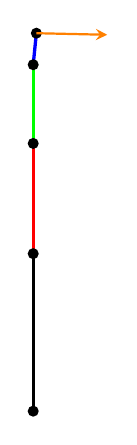
\begin{tikzpicture}[scale=2, >=stealth]
\coordinate (O) at (0,0);
\coordinate (A) at (0,1.0);
\coordinate (B) at (0,1.7);
\coordinate (C) at (0,2.2);
\coordinate (D) at (0.02,2.40);
\draw[black, very thick] (O) -- (A);
\draw[red,   very thick] (A) -- (B);
\draw[green, very thick] (B) -- (C);
\draw[blue,  very thick] (C) -- (D);
\foreach \p in {O,A,B,C,D}{
    \fill (\p) circle (1pt);
}
\draw[->, orange, thick] (D) -- ++(0.45,-0.01);
\end{tikzpicture}
\vspace{3pt}

\(\dot{q} = (1,0,0)\)
\end{minipage}
\hfill
% ----------------- Second figure -----------------
\begin{minipage}{0.32\textwidth}
\centering
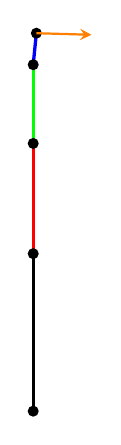
\begin{tikzpicture}[scale=2, >=stealth]
\coordinate (O) at (0,0);
\coordinate (A) at (0,1.0);
\coordinate (B) at (0,1.7);
\coordinate (C) at (0,2.2);
\coordinate (D) at (0.02,2.40);
\draw[black, very thick] (O) -- (A);
\draw[red,   very thick] (A) -- (B);
\draw[green, very thick] (B) -- (C);
\draw[blue,  very thick] (C) -- (D);
\foreach \p in {O,A,B,C,D}{
    \fill (\p) circle (1pt);
}
\draw[->, orange, thick] (D) -- ++(0.35, -0.01);
\end{tikzpicture}
\vspace{3pt}

\(\dot{q} = (0,1,0)\)
\end{minipage}
\hfill
% ----------------- Third figure -----------------
\begin{minipage}{0.32\textwidth}
\centering
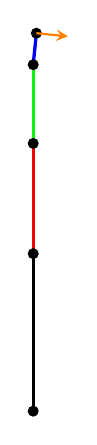
\begin{tikzpicture}[scale=2, >=stealth]
\coordinate (O) at (0,0);
\coordinate (A) at (0,1.0);
\coordinate (B) at (0,1.7);
\coordinate (C) at (0,2.2);
\coordinate (D) at (0.02,2.40);
\draw[black, very thick] (O) -- (A);
\draw[red,   very thick] (A) -- (B);
\draw[green, very thick] (B) -- (C);
\draw[blue,  very thick] (C) -- (D);
\foreach \p in {O,A,B,C,D}{
    \fill (\p) circle (1pt);
}
\draw[->, orange, thick] (D) -- ++(0.2,-0.02);
\end{tikzpicture}
\vspace{3pt}

\(\dot{q} = (0,0,1)\)
\end{minipage}
\end{figure}
\noindent
The robot is \textbf{close to a singularity}, the three velocity vectors become nearly parallel, so the end-effector can barely move in the y-direction.

\subsubsection*{iii) \quad $q_3 = (-\frac{\pi}{2},\frac{\pi}{2},0)^T$}
\begin{figure}[h!]
\centering
% ----------------- First figure -----------------
\begin{minipage}{0.32\textwidth}
\centering
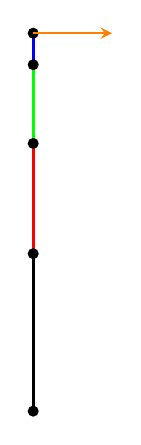
\begin{tikzpicture}[scale=2, >=stealth]
\coordinate (O) at (0,0);
\coordinate (A) at (0,1.0);
\coordinate (B) at (0,1.7);
\coordinate (C) at (0,2.2);
\coordinate (D) at (0,2.4);
\draw[black, very thick] (O) -- (A);
\draw[red,   very thick] (A) -- (B);
\draw[green, very thick] (B) -- (C);
\draw[blue,  very thick] (C) -- (D);
\foreach \p in {O,A,B,C,D}{
    \fill (\p) circle (1pt);
}
\draw[->, orange, thick] (D) -- ++(0.5,0);
\end{tikzpicture}
\vspace{3pt}

\(\dot{q} = (1,0,0)\)
\end{minipage}
\hfill
% ----------------- Second figure -----------------
\begin{minipage}{0.32\textwidth}
\centering
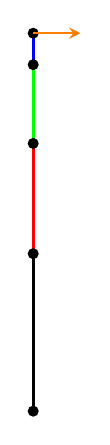
\begin{tikzpicture}[scale=2, >=stealth]
\coordinate (O) at (0,0);
\coordinate (A) at (0,1.0);
\coordinate (B) at (0,1.7);
\coordinate (C) at (0,2.2);
\coordinate (D) at (0,2.4);
\draw[black, very thick] (O) -- (A);
\draw[red,   very thick] (A) -- (B);
\draw[green, very thick] (B) -- (C);
\draw[blue,  very thick] (C) -- (D);
\foreach \p in {O,A,B,C,D}{
    \fill (\p) circle (1pt);
}
\draw[->, orange, thick] (D) -- ++(0.3,0);
\end{tikzpicture}
\vspace{3pt}

\(\dot{q} = (0,1,0)\)
\end{minipage}
%
\hfill
%
% ----------------- Third figure -----------------
\begin{minipage}{0.32\textwidth}
\centering
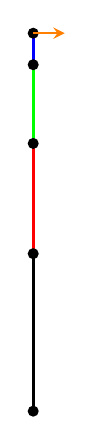
\begin{tikzpicture}[scale=2, >=stealth]
\coordinate (O) at (0,0);
\coordinate (A) at (0,1.0);
\coordinate (B) at (0,1.7);
\coordinate (C) at (0,2.2);
\coordinate (D) at (0,2.4);
\draw[black, very thick] (O) -- (A);
\draw[red,   very thick] (A) -- (B);
\draw[green, very thick] (B) -- (C);
\draw[blue,  very thick] (C) -- (D);
\foreach \p in {O,A,B,C,D}{
    \fill (\p) circle (1pt);
}
\draw[->, orange, thick] (D) -- ++(0.2,0);
\end{tikzpicture}
\vspace{3pt}

\(\dot{q} = (0,0,1)\)
\end{minipage}
\end{figure}
\noindent
The robot is \textbf{in a singularity} configuration, the robot can still move in the x-direction, but it has lost the ability to move in the y-direction.

\section*{B. Trajectory Generation in Joint Space}
\subsection*{1.Generation of smooth trajectories with polynomial splines}
The goal is to generate a smooth joint–space trajectory that starts at


\[
q_a = \begin{bmatrix}0 \\ 0 \\ 0\end{bmatrix},
\]
passes through the via–point
\[
q_b = \begin{bmatrix}-\frac{\pi}{4} \\[2pt] \frac{\pi}{2} \\ 0\end{bmatrix}
\quad \text{at } t=2.5\ \text{s},
\]
and reaches the final configuration
\[
q_c = \begin{bmatrix}-\frac{\pi}{2} \\[2pt] \frac{\pi}{4} \\ 0\end{bmatrix}
\quad \text{at } t=5\ \text{s}.
\]

Each spline segment is defined as a cubic polynomial,
\[
q_{s}(t)=a_0 + a_1 (t-t_{start}) + a_2 (t- t_{start})^2 + a_3 (t_{start})^3,
\]
with $t_{\text{start}} = 0$ and $s$ as a parameter for the corresponding segment. Each q has it's own $q_{s}$.

From that the following conditions result:
\[
    q_0(0) = q_a \quad
    q_0(2.5)= q_b\quad
    \dot q_0(0) = 0 
\]
\[
    \dot q_0(2.5) =
\begin{cases}
\text{0}, & \text{direction does change} \\
\text{Average v of each segment}, & \text{otherwise} \\
\end{cases}
\]
\[
    q_1(2.5) = q_b\quad
    q_1(5) = q_c \quad
\]
\[
    \dot q_1(2.5) =
\begin{cases}
\text{0}, & \text{direction does change} \\
\text{Average v of each segment}, & \text{otherwise} \\
\end{cases}
\]
\[
    \dot q_0(5) = 0 
\]

That means, for each segments we have four conditions. This is a linear systems of equations. We can solve that with python and the library numpy!

\begin{lstlisting}[language=python, breaklines=true, breakatwhitespace=true]
    import numpy as np
from numpy import pi
import matplotlib.pyplot as plt

t_start = 0
t1 = 2.5 
tf = 5.0  

q_a = np.array([0.0, 0.0, 0.0])
q_b = np.array([-pi / 4, pi / 2, 0.0])
q_c = np.array([-pi / 2, pi / 4, 0.0])

v_avg_1 = (q_b - q_a) / t1
v_avg_2 = (q_c - q_b) / (tf - t1)

q_dot_a = np.zeros(3)
q_dot_b = np.zeros(3)
q_dot_c = np.zeros(3)

for i in range(3):
    v1 = v_avg_1[i]
    v2 = v_avg_2[i]

    if (v1 * v2 < 0):
        q_dot_b[i] = 0.0
    else:
        q_dot_b[i] = (v1 + v2) / 2

A_params = np.zeros((3, 2, 4)) 



# What is known: q(0), q(2,5), q'(0), q'(2,5) (first segment)

M_s = np.zeros((3, 2, 4, 4))
V_s = np.zeros((3,2,4))
S_s = np.zeros((3,2,4))

def q(t):
    # q(t)  = a1 + a2 * t + a3*t**2 + a4*t**3
    return np.array([1, t, t**2, t**3])

def q_dot(t):
    # q'(t) = 0 * a1 + a2 + 2*a3*t + 3*a4*t**2
    return np.array([0, 1, 2*t, 3*t**2])



for j in range(3):
    M_s[j][0] = np.array([q(0),q(2.5),q_dot(0),q_dot(2.5)])
    V_s[j][0] = np.array([q_a[j], q_b[j], q_dot_a[j], q_dot_b[j]])    

for j in range(3):
    M_s[j][1] = np.array([q(2.5),q(5),q_dot(2.5),q_dot(5)])
    V_s[j][1] = np.array([q_b[j], q_c[j], q_dot_b[j], q_dot_c[j]])  
    

# solve the equations:
for j in range(3):
    for s in range(2):
        M_s_inv = np.linalg.inv(M_s[j][s])
        S_s[j][s] = M_s_inv  @ V_s[j][s]


\end{lstlisting}
\newpage
Here are the solution vectors for segment 1, each entry in the vector corresponds to a joint:

\[
a_0 = 
\begin{pmatrix}
0.0 \\
0.0 \\
0.0
\end{pmatrix}
\qquad
a_1 = 
\begin{pmatrix}
1.40\times 10^{-16} \\
-2.79\times 10^{-16} \\
0.0
\end{pmatrix}
\]

\[
a_2 = 
\begin{pmatrix}
-0.25 \\
0.75 \\
0.0
\end{pmatrix}
\qquad
a_3 = 
\begin{pmatrix}
0.05\\
-0.20 \\
0.0
\end{pmatrix}
\]

Here are the solution vectors for segment 2:
\[
a_0 =
\begin{pmatrix}
-1.57 \\
-2.36 \\
0.0
\end{pmatrix}
\qquad
a_1 =
\begin{pmatrix}
1.26 \\
3.77 \\
0.0
\end{pmatrix}
\]

\[
a_2 =
\begin{pmatrix}
-0.50 \\
-1.13 \\
0.0
\end{pmatrix}
\qquad
a_3 =
\begin{pmatrix}
0.05 \\
0.10 \\
0.0
\end{pmatrix}
\]

In \ref{fig:joint_trajectories} you can see $q_t$ for each joint with respect to time.

\begin{figure}[h]
  \centering

  \begin{minipage}[b]{0.8\textwidth}
    \centering
    
\includegraphics[width=\textwidth]{A2/imgs/joint_trajectories.png}
    \caption{Graph of $q_t$ for each joint with respect to time}
    \label{fig:joint_trajectories}
  \end{minipage}
  \hfill


\end{figure}


% ------------------------------------------------------------
% \paragraph{Velocity conditions at the via–point.}

% \begin{itemize}
%     \item \textbf{Joint 1} moves monotonically
%     \(
%     0 \rightarrow -\frac{\pi}{4} \rightarrow -\frac{\pi}{2},
%     \)
%     so the velocity at the via–point should be non-zero.  
%     The average velocity is  
%     \[
%     v_{\mathrm{avg}} = 
%     \frac{-\frac{\pi}{4}-0}{2.5}
%     = -\frac{\pi}{10}
%     \approx -0.314.
%     \]
%     \item \textbf{Joint 2} reverses its direction 
%     \(
%     0 \rightarrow \frac{\pi}{2} \rightarrow \frac{\pi}{4}.
%     \)
%     To avoid a sharp corner in the trajectory, the via–point velocity is set to  
%     \[
%     \dot q_2(2.5)=0.
%     \]
%     \item \textbf{Joint 3} remains at zero for all times; therefore  
%     \[
%     \dot q_3(t)=0 \quad \forall t.
%     \]
% \end{itemize}

% % ------------------------------------------------------------
% \paragraph{Cubic Spline Segment 1 ($0\le t\le2.5$).}\
% Boundary conditions:
% \[
% q(0)=q_a,\quad q(2.5)=q_b,\quad 
% \dot q(0)=0,\quad \dot q(2.5)=v_{\mathrm{via}}.
% \]

% Solving the cubic polynomial yields (rounded to two decimals):
% \[
% a_0^{(1)}=
% \begin{bmatrix}0\\0\\0\end{bmatrix},\quad
% a_1^{(1)}=
% \begin{bmatrix}0\\0\\0\end{bmatrix},
% \]
% \[
% a_2^{(1)}=
% \begin{bmatrix}-0.25\\ 0.75\\ 0\end{bmatrix},\qquad
% a_3^{(1)}=
% \begin{bmatrix}0.06\\ -0.30\\ 0\end{bmatrix}.
% \]

% Thus,
% \[
% q(t)=
% \begin{bmatrix}
% -0.25\, t^2 + 0.06\, t^3 \\[4pt]
% \ \ 0.75\, t^2 - 0.30\, t^3 \\[4pt]
% 0
% \end{bmatrix}, \qquad 0\le t\le 2.5.
% \]

% % ------------------------------------------------------------
% \paragraph{Cubic Spline Segment 2 ($2.5 < t\le 5$).}\


% Boundary conditions:\[
% q(2.5)=q_b,\quad q(5)=q_c,\quad 
% \dot q(2.5)=v_{\mathrm{via}},\quad \dot q(5)=0.
% \]

% The resulting coefficients are
% \[
% a_0^{(2)}=
% \begin{bmatrix}
% -0.79 \\ 1.57 \\ 0
% \end{bmatrix},\quad
% a_1^{(2)}=
% \begin{bmatrix}
% -0.31 \\ 0 \\ 0
% \end{bmatrix},
% \]
% \[
% a_2^{(2)}=
% \begin{bmatrix}
% 0.38 \\ -1.51 \\ 0
% \end{bmatrix},\qquad
% a_3^{(2)}=
% \begin{bmatrix}
% -0.10 \\ 0.60 \\ 0
% \end{bmatrix}.
% \]

% Thus,
% \[
% q(t)=
% a_0^{(2)} + a_1^{(2)} t + a_2^{(2)} t^2 + a_3^{(2)} t^3,
% \qquad 2.5 < t \le 5.
% \]


\subsection*{2. Trajectories in joint space}
In the following section we will explain how we make sure that $v_{max}$ and $a_{max}$ is not exceeded. Again we have for each joint one function $q$ that is describing the trajectory of the joint over time. We also know the first two derivations.

\[
q(t) = a_0 + a_1\, t + a_2\, t^2 + a_3\, t^3
\]

\[
\dot{q}(t) = a_1 + 2 a_2\, t + 3 a_3\, t^2
\]

\[
\ddot{q}(t) = 2 a_2 + 6 a_3\, t
\]

However, we have again four conditions for our parameters $a_0, ..., a_3$.

\begin{align*}
q(t_s) &= q_0 \\
\dot{q}(t_s) &= 0 \\
q(t_f) &= q_f \\
\dot{q}(t_f) &= 0
\end{align*}

When do equivalent transformation then we can get formulars for $a_0, ..., a_3$
\[
a_0 = q_0, \quad a_1 = 0, \quad a_2 = \frac{3}{t_f^2}(q_f - q_0), \quad a_3 = -\frac{2}{t_f^3}(q_f - q_0)
\]

Now we have to ask the question how to choose $tf$ such that we are not exceeding $v_{max}$ and $a_{max}$. In order to achieve that we are defining an additional condition:

\[
|\dot{q}(t) |\leq v_{\text{max}} \quad \land \quad |\ddot{q}(t) |< a_{\text{max}}
\]

Due to the fact that $\dot{q}(t)$ is a quadratic function and symmetric, we can follow that the global maximum of $\dot{q}(t)$ for $t \in [t_s, t_f] $ is at $t=t_f/2$. The function $\ddot{q}(t)$ is linear, thus the global maximum is at $t=0$ and $t=t_f$ ($|\ddot{q}(0)| = |\ddot{q}(t_f)|$). When we do term forming we get:

\[
\left| \frac{3}{2 v_{\text{max}}} \Delta q \right| \leq t_f \quad \land \quad \sqrt{\left| \frac{6 \Delta q}{a_{\text{max}}} \right|} \leq t_f
\]

Where $\Delta q = q_f - q_0$. To satisfy both conditions, we just take the maximum value.

\[
\max \left( \left| \frac{3}{2 v_{\text{max}}} \Delta q \right|, \sqrt{\left| \frac{6 \Delta q}{a_{\text{max}}} \right|} \right)
\]

That must be done for every q(t) that corresponds to a joint. That is the idea of the code. However, in order to make sure that every joint is done with its movement at the same time, we have to take the largest $t_f$ over all joints.
\\

In \ref{fig:dq}, \ref{fig:q} and \ref{fig:tau} you can see the plots for execution the proj1control function. The chosen gains are the following:

\[
\mathbf{k}_p = \begin{pmatrix} 400 \\ 400 \\ 400 \end{pmatrix}, \quad \mathbf{k}_v = \begin{pmatrix} 40 \\ 40 \\ 40 \end{pmatrix}
\]

\begin{figure}[h]
  \centering

  \begin{minipage}[b]{0.5\textwidth}
    \centering
    
\includegraphics[width=\textwidth]{A2/imgs/tau.png}
    \caption{$\tau$ for each joint with respect to time}
    \label{fig:tau}
  \end{minipage}
  \hfill


\end{figure}


\begin{figure}[h]
  \centering

  \begin{minipage}[b]{0.5\textwidth}
    \centering
    
\includegraphics[width=\textwidth]{A2/imgs/q.png}
    \caption{$q$ for each joint with respect to time}
    \label{fig:q}
  \end{minipage}
  \hfill


\end{figure}

\begin{figure}[h]
  \centering

  \begin{minipage}[b]{0.5\textwidth}
    \centering
    
\includegraphics[width=\textwidth]{A2/imgs/dq.png}
    \caption{$dq$ for each joint with respect to time}
    \label{fig:dq}
  \end{minipage}
  \hfill


\end{figure}
\newpage
\section*{C. Operational Space Control}
\subsection*{1.Project 2 - Circle}
\textit{control.cpp}


\subsection*{2.Project 2 - Control}
\textit{control.cpp}


\subsection*{3.Project 2 - Gain tuning and plots }
Figures \ref{fig:tuned} and \ref{fig:tuned_traj} show different values for the circle trajectory with the tuned controller. For higher Kp the trajectory is tracked better, so $x-x_d$ shows lower values, and the spike in error at the start of the trajectory looks more pointy. In addition, there is a higher output force $\tau$ at the beginning of the trajectory since the reference starts at a high velocity directly. For lower Kp, the spike in the error at the beginning of the trajectory is smoother but the average tracking error is higher.

\begin{figure*}[h]
  \centering

  \begin{minipage}[b]{0.9\textwidth}
    \centering
    \subfloat[$q_s$]{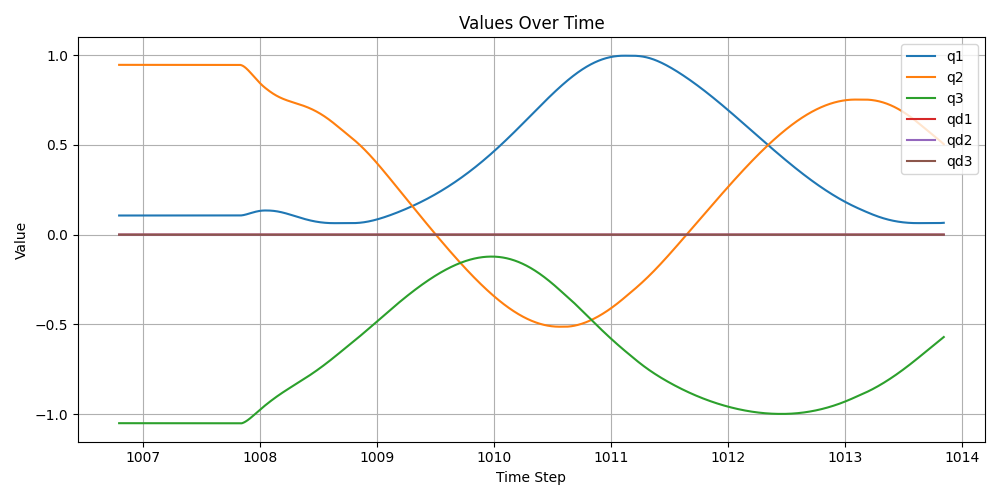
\includegraphics[width=0.45\textwidth]{imgs/qs.png}} \hfill
    \subfloat[$\tau$]{
\includegraphics[width=0.45\textwidth]{imgs/taus.png}} \hfill
    \subfloat[$x$]{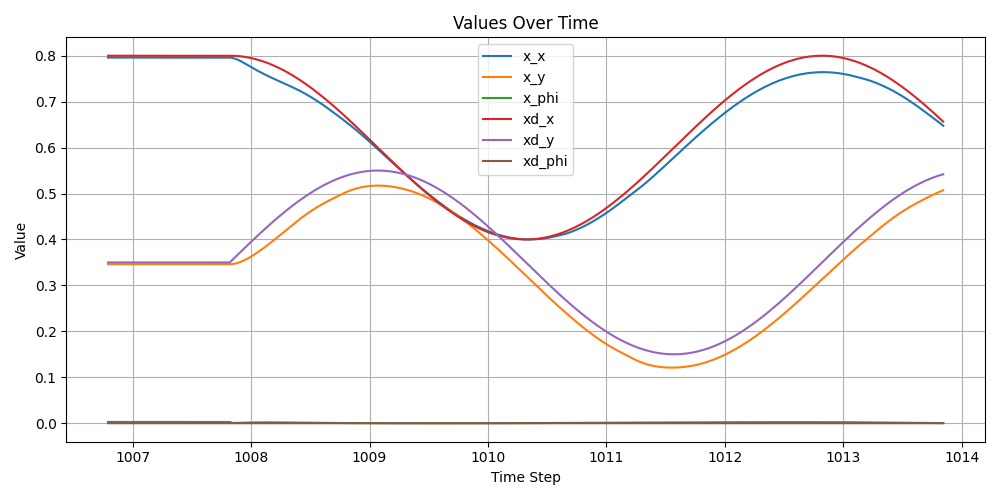
\includegraphics[width=0.45\textwidth]{imgs/x_xd.png}} \hfill
    \subfloat[$x-x_d$]{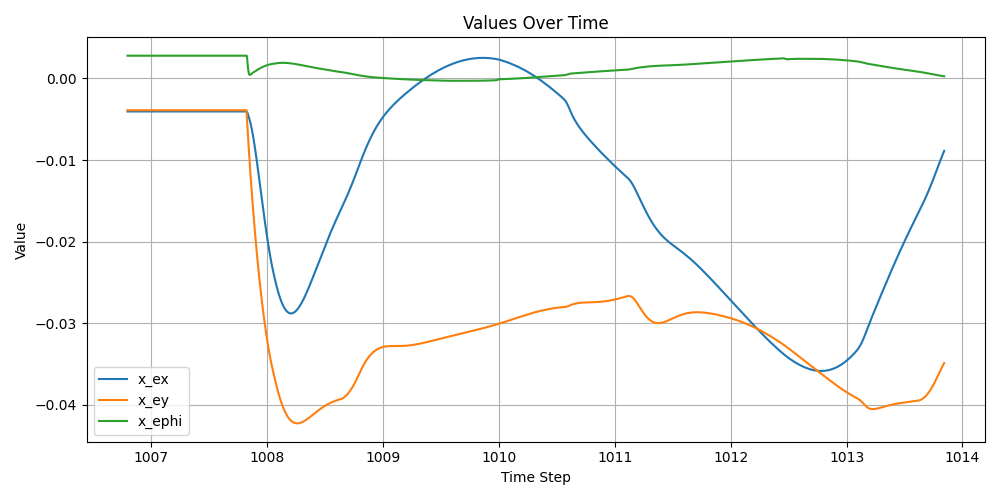
\includegraphics[width=0.45\textwidth]{imgs/e.png}}
    \caption{Kp: 5000, 5000, 4000, Kd: 400, 400, 40}
    \label{fig:tuned}
  \end{minipage}

\end{figure*}

\begin{figure*}[h]
  \centering

  \begin{minipage}[b]{0.9\textwidth}
    \centering
    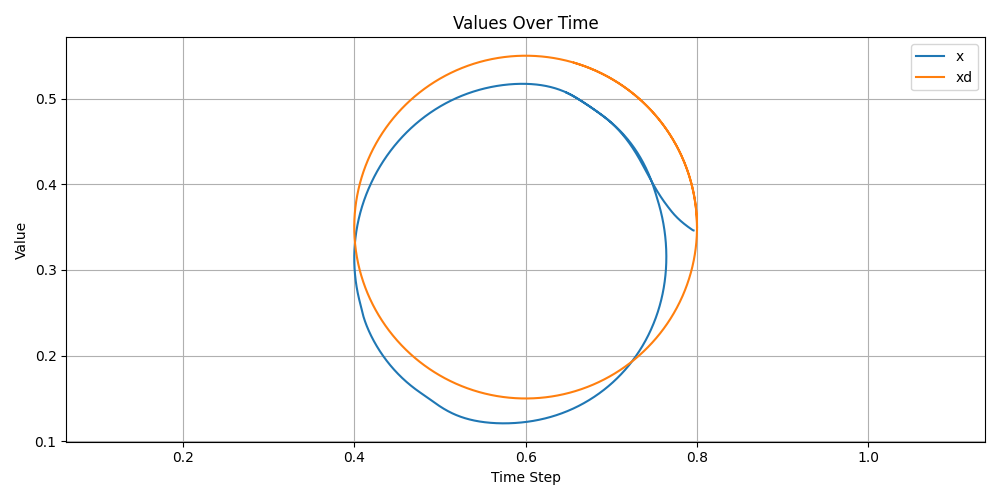
\includegraphics[width=0.7\textwidth]{imgs/traj.png}
    \caption{XY-plane visualization of the desired end-effector trajectory and the real trajectory. Kp: 5000, 5000, 4000, Kd: 400, 400, 40}
    \label{fig:tuned_traj}
  \end{minipage}

\end{figure*}

%\begin{figure}[h]
%  \centering
%
%  \begin{minipage}[b]{0.3\textwidth}
%    \centering
%    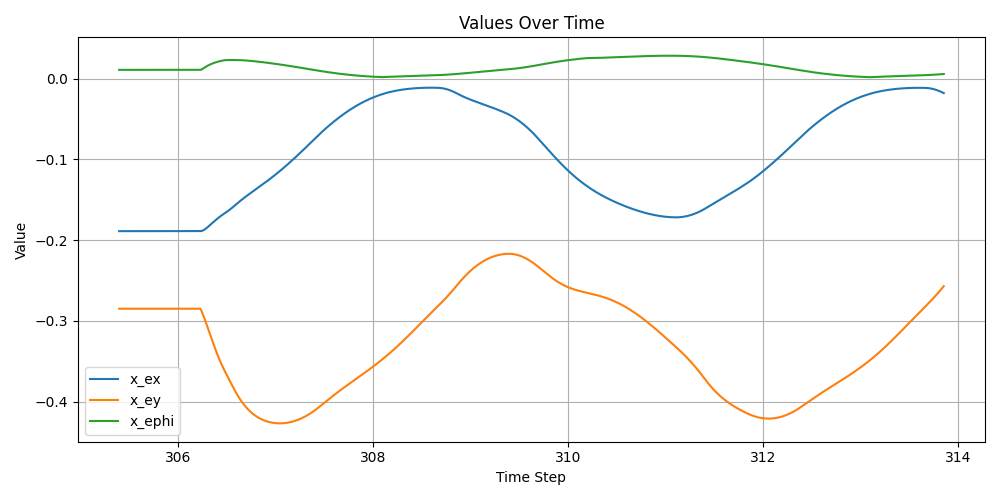
\includegraphics[width=\textwidth]{imgs/kp_small.png}
%    \caption{Kp: 500, 300, 150}
%    \label{fig:kp_small}
%  \end{minipage}
%  \hfill
%  \begin{minipage}[b]{0.3\textwidth}
%    \centering
%    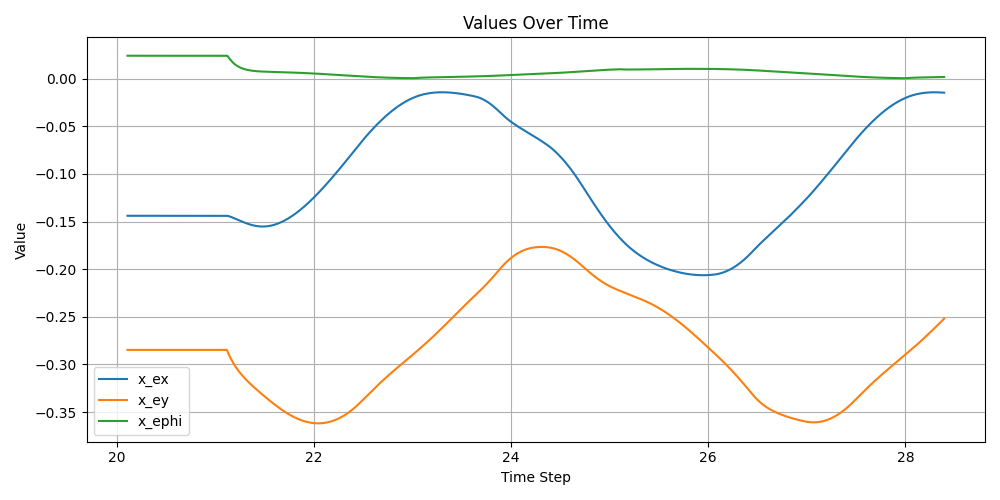
\includegraphics[width=\textwidth]{imgs/kp_normal.png}
%    \caption{Kp: 600, 400, 200}
%    \label{fig:kp_normal}
%  \end{minipage}
%  \hfill
%  \begin{minipage}[b]{0.3\textwidth}
%    \centering
%    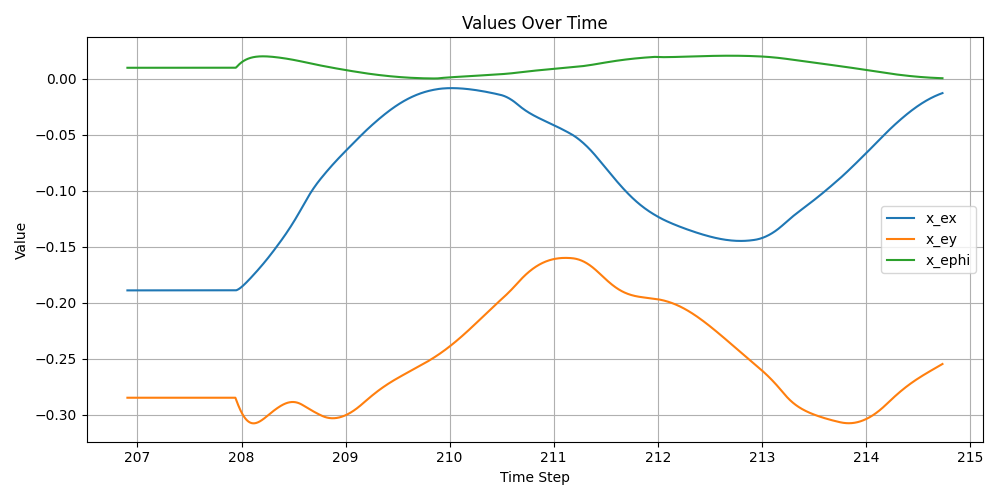
\includegraphics[width=\textwidth]{imgs/kp_large.png}
%    \caption{Kp: 700, 500, 250}
%    \label{fig:kp_large}
%  \end{minipage}
%
%\end{figure}


\subsection*{4.Project 3 - Parabolic Blends}
Figure \ref{fig:para_traj} shows the desired $\beta$ and $\dot{\beta}$ values for the circle trajectory using the parabolic blends method. This method ensures that the reference trajectory slowly increases the desired velocity instead of setting a high velocity directly, which is physically impossible.

\begin{figure*}[h]
  \centering

  \begin{minipage}[b]{0.9\textwidth}
    \centering
    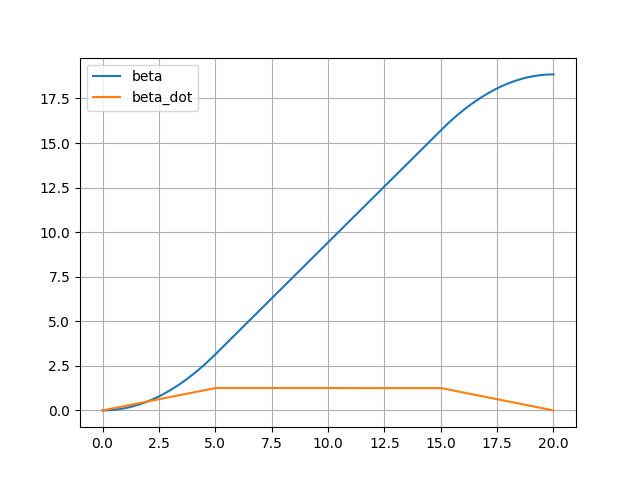
\includegraphics[width=0.7\textwidth]{imgs/betas.png}
    \caption{Desired $\beta$ and $\dot{\beta}$ for the Parabolic Blends method.}
    \label{fig:para_traj}
  \end{minipage}

\end{figure*}


\subsection*{5.Optional}




\noindent\textbf{Contributions:}

\end{document}
